\documentclass[12pt]{beamer}
\usepackage{beamerthemeHannover, graphicx, clrscode, amsmath, amssymb, multicol}
\usepackage{textcomp} \usepackage{verbatim}
\usepackage{listings}
\setbeamercolor{sidebar}{use=structure,bg=gray!60!green}
\lstset{language=SQL}

\title{Doing The Jitterbug \\ \small {Cross Language Continuous Integration for Git} }
\author[@dukeleto]{Jonathan "Duke" Leto}
\date{}

\begin{document}

\frame{
    \titlepage
    \begin{center}
    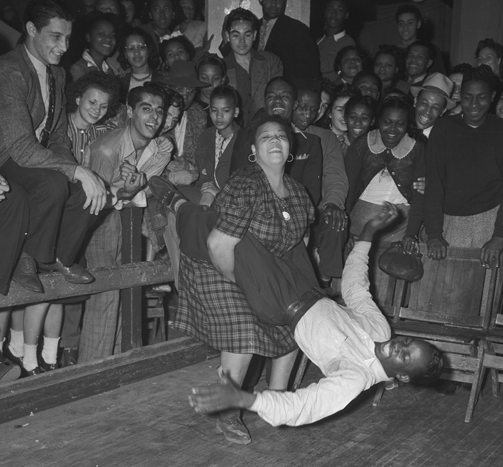
\includegraphics[width=125px, height=115px]{dancing.jpg}
    \end{center}
}

\frame{
    \frametitle{What is Continuous Integration (CI) ?}

    Continually and automatically testing code, usually with relevant notifications.
}

\frame{
    \frametitle{Why is CI Useful?}
    \begin{itemize}
        \item Know the exact commit that broke something
        \item Automate testing many different combinations of different versions
            of libraries, languages, OS's, browsers, etc...
        \item Quickly identifies tests that only pass on the authors machine
            due to implicit assumptions
    \end{itemize}
}

\frame{
    \frametitle{What problems does Jitterbug solve?}
    \begin{itemize}
        \item People forgetting to run the test suite
        \item People forgetting to notify others when they see breakage
        \item Not having a visual interface to which commits passed
            and which failed a test suite
    \end{itemize}
}

\frame{
    \frametitle{What does Jitterbug look like?}

    \begin{center}
        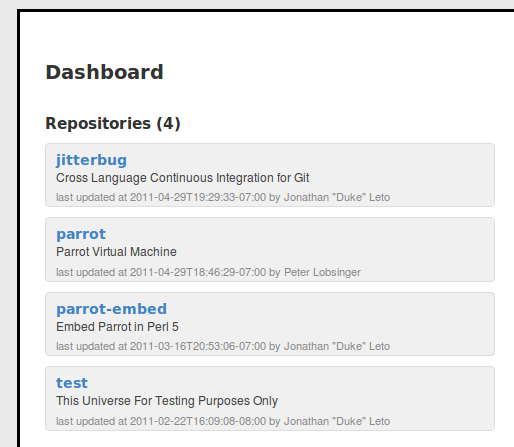
\includegraphics[width=260px, height=225px]{jitterbug_dashboard}
    \end{center}
}

\frame{
    \frametitle{What does Jitterbug look like? (2)}

    \begin{center}
        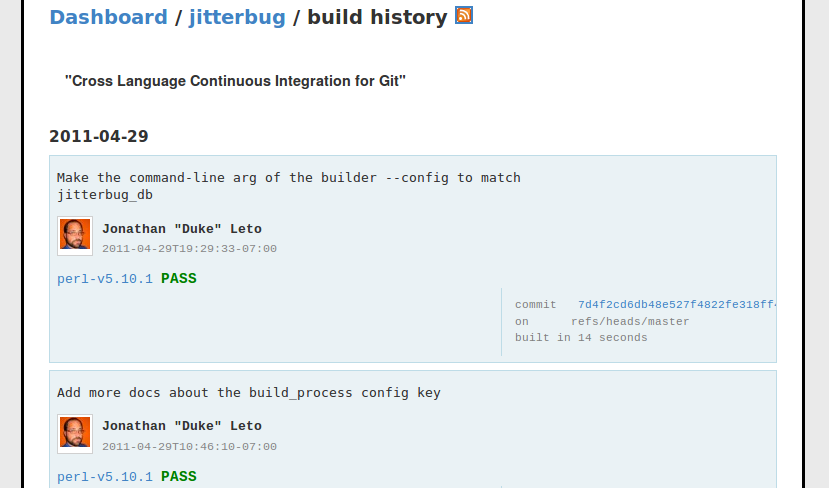
\includegraphics[scale=0.3]{jitterbug_project}
    \end{center}
}

\frame{
    \frametitle{What does Jitterbug look like? (3)}
    \begin{center}
        
\includegraphics[scale=0.3]{jitterbug_email}
    \end{center}
}

\frame{
    \frametitle{Current Features}
    \begin{itemize}
        \item Integrates seamlessy with Github post-receive hooks
        \item Can run tests for Perl 5/6, Parrot, Ruby and Makefile-based projects
        \item Highly customizable YAML configuration file
        \item Email notifier
        \item Supports custom build/test scripts
        \item Pretty web interface
    \end{itemize}
}


\frame{
    \frametitle{Getting Jitterbug}
    \begin{itemize}
        \item  git clone git://github.com/franckcuny/jitterbug.git
        \item cd jitterbug
        \item perl Build.PL
        \item ./Build installdeps \# install dependencies
        \item ./Build test        \# run tests
    \end{itemize}

    Will release to CPAN Real Soon Now
}

\frame{
    \frametitle{Doing the Jitterbug}
    \begin{itemize}
        \item vi config.yml \# Customize YAML config
        \item perl jitterbug.pl -p 8080 \# Web interface
        \item perl scripts/jitterbug\_db --config config.yml --deploy
        \item perl scripts/builder.pl -c config.yml
        \item Add http://example.com:8080/hook/ as a Github post-receive URL
    \end{itemize}
}

\frame{
    \frametitle{Customizing Jitterbug}
    Interesting config file options...
    \begin{itemize}
        \item reuse\_repo - Reuse git repos instead of recloning
        \item stack\_tasks - Test every commit, not just current HEAD
        \item perlbrew - use perlbrew to test under many versions/builds of Perl
        \item email\_on\_pass - whether to send emails for PASSing test suites
    \end{itemize}
}

\frame{
    \frametitle{Future Goals}
    \begin{itemize}
        \item Jitterbug wants to support running tests in many more languages, including
        \begin{itemize}
            \item Python
            \item Javascript
            \item PHP
        \end{itemize}
        \item Code coverage
        \item Graphic visualization
    \end{itemize}
}

\frame{
    \frametitle{Get involved!}
    \begin{itemize}
        \item Install Jitterbug and test your projects
        \item Join \#dancer on irc.perl.org for help
        \item Submit a pull request for an issue! https://github.com/franckcuny/jitterbug
        \item http://lumberjaph.net/jitterbug
    \end{itemize}
}

\frame{
    \frametitle{ Thanks! }
    \begin{itemize}
        \item Franck Cuny
        \item Boyce Thompson Institute for Plant Research
    \end{itemize}
}

\frame{
    \frametitle{ Stalk Me }
    \begin{center}
        \begin{itemize}
           \item http://leto.net
           \item @dukeleto / !leto on twitter/identi.ca
           \item http://linkedin.leto.net
           \item Slides available at http://github.com/leto/presentations
        \end{itemize}
    \end{center}
}
\end{document}
